\subsection{Integration of the Radiation Transfer Equation}

\begin{figure}[h]
	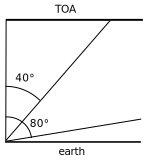
\includegraphics[width=10cm]{figures/geometry.png}
	\caption{"Geometry of the athmosphere"}
	\label{fig:geometry}
\end{figure}

The intensity in \eqn{eqn1} is integrated along a path from the earth surface to the TOA (top of athmosphere) which is assumed to be at a heigth of $70 km$. Assuming constant $\kappa$ and $\epsilon$ in \eqn{eqn1} the solution is given by:
\begin{align}
	I(s) = I(s_0) \exp( -  \kappa (s-s_0)) +  \dfrac{\epsilon}{\kappa} \left(1 - \exp( - \kappa (s-s_0))\right)
\end{align}
Because $\kappa$ and $\epsilon$ are not constant along the path from earths surface to TOA the inegration is subdivided into many steps. At each step $\kappa$ and $\epsilon$ are aclculated using local values of temperature and density.

In order to compute the total irradiance emenating from an area element of the surface to TOA the integration has to be done over the half sphere:
\begin{align}
	F(\theta) &= \int_0^{2 \pi} \int_0^{\pi/2} I(\theta) \sin(\theta) \cos(\theta)  d \theta d \phi \\
	  &= 2 \pi \int_0^{\theta} I(\theta) \sin(\theta) \cos(\theta) d \theta
\end{align}
The intensity $I(\theta)$ is computed at $0^o$ and two further angles (in the computations $40^o$ and $80^o$ are chosen), 
the intermedite values are interpolated by a cubic polnomial (\chap{app_a_2}).
After determining the polynomial cofficients:
\begin{align}
	a_2 &= \dfrac{(F_1 - F_0) \theta_2^3 - (F_2 - F_0) \theta_1^3}{\theta_1^2 \theta_2^3 - \theta_1^3 \theta_2^2} \\
	a_3 &= \dfrac{(F_2 - F_0) \theta_1^2 - (F_1 - F_0) \theta_2^2}{\theta_1^2 \theta_2^3 - \theta_1^3 \theta_2^2}
 \end{align}  
the integral is given by:
\begin{align}
	F(\theta) &= 2 \pi \int_0^{\theta} \left(a_0 + a_2 \theta^2 + a_3 \theta^3\right) \sin(\theta) \cos(\theta)  d \theta d \phi
\end{align}
The contributions of the different polynomial orders assuming constant $I(\theta)$ are:
\begin{align*}
	 &\int_0^{\theta} \sin(\theta) \cos(\theta) d \theta = 0.5 \\
	 &\int_0^{\theta} \theta^2 \sin(\theta) \cos(\theta) d \theta = 0.37  \\
	 &\int_0^{\theta} \theta^3 \sin(\theta) \cos(\theta) d \theta = 0.38
\end{align*}

\subsection{The HITRAN Data}

The spectroscopic $CO_2$ data where taken from the HIRAN database (\cite{hitran1}). The standard HITRAN data files use a fixed size format and information that are not used in the present report. HITRAN allows to define ones own format and data output. For easier handling the entries are seperated by commas. The data rows are composed of: 
\begin{enumerate}
	\item Molecule ID, for $CO_2$ this is $2$			
 	\item Isotopologue ID, for $CO_2$ $1-9$			
 	\item the transition wavenumber $\nu$	[$cm^{-1}$]		
    \item the line strength multiplied by isotopologue abunadance $S$, [$cm^{-1}/(molec \;cm^{-2}$]		
 	\item Einstein coefficient of spontaneous emission $A$ [$s^{-1}$]		
 	\item pressure line broadeing coefficient by collisions with air molecules $\gamma_{air}$ [$cm^{-1} atm^{-1}$]		
 	\item pressure line broadeing coefficient by collisions with $CO_2$ molecules $\gamma_{self}$ [$cm^{-1} atm^{-1}$]		
	\item energy of the lower state $E"$ [$cm^{-1}$]		
	\item temperature exponent $n_{air}$ for the air broadened HWHM			
	\item pressure shift induced by air $\delta_{air}$, referred to $p = 1 atm$ [$cm^{-1} atm^{-1}$] 		
	\item upper state degeneracy $g'$			
	\item upper state degeneracy $g"$
\end{enumerate}
In the present report wavelenght $\lambda$ [$m$] and energy [$J$] is used, whereas HITRAN uses wavenumber [$cm^{-1}$]. The transition from wavelenth to wavenumber has to be done carefully.  
\begin{align*}
	\lambda_{ul}     & \leftarrow \dfrac{10^{-2}}{\nu}               & [m]                   \\
	\Delta E_{ul}    & \leftarrow \dfrac{h  c}{\lambda_{ul}}         & [J]                   \\
 	E_l              & \leftarrow h  c  \dfrac{E''}{10^{-2}}         & [J]                   \\
	E_u              & \leftarrow E_l + \Delta E_ul                  & [J]                   \\
	\gamma_a         & \leftarrow \dfrac{\gamma_{air}}{10^{-2}}  10^{-5} & \left[\dfrac{1}{m \; Pa}\right] \\
	\gamma_s         & \leftarrow \dfrac{\gamma_{self}}{10^{-2}}  10^{-5} & \left[\dfrac{1}{m \; Pa}\right] \\
	\delta_a         & \leftarrow \dfrac{\delta_{air}}{10^{-2}}  10^{-5} &
\end{align*}

The HWHM Doppler line broadening is given by: 
\begin{align*}
	\alpha_D(T) = \dfrac{\nu_{ij}}{c} \sqrt{\dfrac{2 N_A k T \ln 2}{M}}
\end{align*}
The temperatue and pressure dependence of pressure broadened line width and pressure shift are defined by HITRAN as follows \cite{hitran2}: 
\begin{align*}
	\gamma(p, T) &= \left(\dfrac{T_{ref}}{T}\right)^{n_{air}}  
	               \left(  \gamma_{air} (p_{ref}, T_{ref}) (p - p_{self}) +
	                       \gamma_{self}(p_{ref}, T_{ref}) p_{self}  \right) 		 \\
	\nu_{ij}^*   &= \nu_{ij} \delta(p_{ref}) p
\end{align*}

Temperature dependent partition functions can be found at \cite{hitran3}.